\documentclass{article}
\usepackage[portuguese]{babel}
\usepackage{graphicx}
\usepackage{float}
\usepackage{hyperref}
\usepackage[onehalfspacing]{setspace}
\usepackage{indentfirst}
\usepackage{amssymb}
\usepackage{amsmath}
\usepackage{amsthm}
\usepackage{mathtools}
\usepackage[thinc]{esdiff}
\usepackage{upgreek}
\usepackage{csquotes}
\usepackage[backend = biber]{biblatex}
\addbibresource{refs.bib}

\usepackage[letterpaper,top=3cm,bottom=2cm,left=3cm,right=2cm,marginparwidth=1.75cm]{geometry}

\title{Dinâmica predador-presa com doenças afetando a população de presas}
\author{Fernanda Luísa Silva Gomes \\ João Lucas Duim}
\date{Setembro de 2021}

\begin{document}
\maketitle

\section{Introdução}
Muitas são as referências onde pode-se encontrar estudos sobre a dinâmica predador-presa e sobre epidemiologia, dado o avanço ocorrido nessas áreas ultimamente. No entanto, ainda são escassas as referências que contemplam a fusão dessas duas importantes áreas de pesquisa. A abordagem desse trabalho mostra-se extremamente útil, visto que nenhuma população real encontra-se completamente invulnerável a epidemias. Apesar disso, a fim de evitar demasiada complexidade dos modelos e também pela escassez de artigos que abordem epidemias em ambas as populações, trataremos o caso em que apenas a população de presas é afetada por epidemias, as quais não afetam a população de predadores pelo ato da predação.

Neste artigo encontra-se uma abordagem essencialmente teórica, não envolvendo análise de nenhum conjunto de dados de situações reais. O sistema eco-epidemiológico descrito terá $3$ atores: o predador, a presa suscetível e a presa infectada. Nesse sistema, nota-se, principalmente, a predação de presas infectadas, visto que a doença a enfraquece, deixando-a mais exposta e vulnerável.

Um dos trabalhos de modelagem sobre o tema, por  Joydev Chattopadhyay e Ovide Arino \cite{chattopadhyay}, assume as mesmas premissas e utiliza uma metodologia semelhante à deste artigo. Além disso, nele é apresentada uma análise matemática minuciosa, permeada por interpretação biológica que produz ricas conclusões, sendo o seguinte resultado de especial interesse para a modelagem aqui apresentada: ``Quando a taxa máxima de renovação da população infectada é menor do que sua taxa de mortalidade natural, então ambas as populações (infectadas e predadoras sãs) vão à extinção.".

Md Sabiar Rahman e Santabrata Chakravarty \cite{rahman} modela o mesmo fenômeno biológico em questão com a premissa adicional de que as presas infectadas são incapazes de se reproduzir. O sistema de equações tratado é:

\begin{equation*}
    \begin{cases}
        \dfrac{dS}{dt} = rS \left( 1 - \dfrac{S + I}{k} \right) - \dfrac{c_1SP^2}{a + (S + I)P} - \lambda IS \\
        \dfrac{dI}{dt} = \lambda IS - \dfrac{c_2IP^2}{a + (S + I)P} - \gamma I \\
        \dfrac{dP}{dt} = \dfrac{e(c_1S + c_2I)P^2}{a + (S + I)P} - dP
    \end{cases}
\end{equation*}
onde $P$, $S$ e $I$ representam, respectivamente, as populações de predadores, presas suscetíveis e presas infectadas. Os parâmetros $r$, $k$, $\lambda$, $c_2$, $c_1$, $a$, $\gamma$, $e$, $d$ pertencem todos a $\mathbb{R}_+$, sendo que $r$ representa a taxa de crescimento da população de presas, $k$ representa a capacidade de suporte do meio, $\lambda$ representa a força da infecção, $c_2$ é a taxa de predação de presas infectadas, $c_1$ é a taxa de predação de presas suscetíveis, $a$ representa a constante de meia saturação, $\gamma$ é a taxa de mortalidade total de presas infectadas (taxa de morte natural + taxa de mortalidade devido à doença), $e$ é o fator de conversão e $d$ representa a taxa de morte natural da população de predadores. Nesta investigação, a delimitação das soluções, a existência e a estabilidade de diferentes equilíbrios foram minuciosamente examinados, sendo de grande valor as conclusões obtidas.

Por fim, Krishna pada Das et al  \cite{pada} apresenta um estudo similar, com o tema ``Um estudo matemático da dinâmica predador-presa com doenças afetando a população de predadores". Assume-se que, na ausência de predadores, a população de presas cresce segunda uma curva logística e que a doença é disseminada apenas entre a população de predadores, segundo a lei de ação das massas. O sistema de equações tratado é:

\begin{equation*}
    \begin{cases}
        \dfrac{dX}{dT} = rX \left( 1 - \dfrac{X}{k} \right) - \dfrac{c_1X(Y + fZ)}{a_1 + X} \\
        \dfrac{dY}{dT} = \dfrac{m_1X(Y + fZ)}{a_1 + X} - d_1Y - \lambda_1 Y Z \\
        \dfrac{dZ}{dT} = \lambda_1 Y Z - (d_1 + a_1) Z
    \end{cases}
\end{equation*}

onde $X$, $Y$ e $Z$ representam, respectivamente, as populações de presa, predador suscetível e predador infectado, $c_1$ é a taxa de predação do predador suscetível, $c_1f$ é a taxa de predação do predador infectado, $\lambda_1$ é a taxa de infecção e $a_1$ é a constante de meia saturação. Este estudo indica que dois resultados muito diferentes são possíveis: a população de predadores infectados pode ser levada à extinção ou atingir um equilíbrio instável. Apesar do trabalho de modelagem feito não ser exatamente sobre o mesmo fenômeno, a metodologia é bastante similar e útil para a confecção do modelo deste artigo.

\section{Metodologia}
Nosso sistema eco-epidemiológico é constituído de três espécies, sendo elas: a presa suscetível, a presa infectada e a população de predadores. De modo a simplificar o problema, assumiremos que a população de presas sãs cresce de acordo com uma lei logística envolvendo toda a população de presas. Além disso, a taxa de transmissão entre a população de presas suscetíveis e infectadas segue a lei simples de ação de massa. A doença se espalha apenas entre a população de presas, estando os predadores imunes, e a doença não é herdada geneticamente. As populações infectadas não se recuperam e não se tornam imunes. Por último, a população de predadores se alimenta principalmente da população de presas infectadas. 

A partir das suposições acimas, obtemos o seguinte sistema de EDOs:
\begin{equation*}
\begin{split}
    \begin{cases}
    \diff{S}{t} & = r(S+I) \left( 1 - \dfrac{S+I}{k} \right) - bSI - \upeta \upgamma_1(S)Y \\
    \diff{I}{t} & = bSI - \upgamma(I)Y - cI \\
    \diff{Y}{t} & = (\varepsilon \upgamma(I) + \upeta \varepsilon \upgamma_1(S) - d)Y
    \end{cases}
\end{split}
\end{equation*}

O parâmetro $r$ é a taxa de crescimento intrínseca da população de presas suscetíveis, $k$ é o suporte do ecossistema ou capacidade de suporte ambiental, $b$ é a taxa de transmissão entre as populações de presas sãs e infectadas, $c$ é a taxa de mortalidade natural das presas infectadas (sem ser devido à predação), $d$ é a taxa de mortalidade da população de predadores, $\varepsilon$ é a taxa de conversão de presas em predadores, e $\upgamma(I)$ e $\upeta \upgamma(S)$ são as respostas funcionais do predador. Vale ressaltar que a resposta funcional quantifica como a taxa de consumo de consumidores individuais muda em função da densidade de recursos. Para fins de simulações, é amplamente utilizada uma resposta funcional do tipo III (sigmóide), na qual a taxa de ataque acelera inicialmente e depois desacelera quando chega ao ponto em que o consumidor fica com a barriga cheia.

\subsection{Compartimento S}
O primeiro compartimento do modelo é o $S$. Esse compartimento representa a população de presas sãs e suscetíveis, ou seja, que não estão contaminadas, mas podem contrair a doença. A população de presas cresce segundo uma lei logística contendo toda a equação das presas. Adicionalmente, as presas passam de suscetíveis para infectadas conforme a lei da ação das massas. Desse modo, a variação desse compartimento é descrita pela equação
\begin{equation*}
    \diff{S}{t} = r(S+I) \left( 1 - \dfrac{S+I}{k} \right) - bSI - \upeta \upgamma_1(S)Y.
\end{equation*}

\subsection{Compartimento I}
O segundo compartimento do modelo é o $I$ que representa a população de presas infectadas. Se uma presa suscetível for infectada, ela permanece infectada até morrer, uma vez que ela não se recupera e não se torna imune. A variação desse compartimento é descrita pela equação
\begin{equation*}
    \diff{I}{t} = bSI - \upgamma(I)Y - cI.
\end{equation*}

\subsection{Compartimento Y}
O último compartimento do modelo é o $Y$. Esse compartimento representa  os predadores. A doença infecta somente as presas, estando a população de predadores imunes. A variação desse compartimento é
\begin{equation*}
    \diff{Y}{t} = (\varepsilon \upgamma(I) + \upeta \varepsilon \upgamma_1(S) - d)Y.
\end{equation*}

\subsection{Análise dimensional}
Visto que estamos trabalhando com populações, sabemos que [S] = [I] = [Y] = [indivíduos]. Assim
\begin{equation*}
    \left[ \diff{S}{t} \right] = \left[ \diff{I}{t} \right] = \left[ \diff{Y}{t} \right] = \left[ \dfrac{\text{indivíduos}}{\text{tempo}}\right].
\end{equation*}

Desse modo, temos
\begin{equation*}
\begin{split}
    \diff{S}{t} & = r(S+I) \left( 1 - \dfrac{S+I}{k} \right) - bSI - \upeta \upgamma_1(S)Y \\
    \left[ \dfrac{\text{indivíduos}}{\text{tempo}} \right] & = [r] \text{[indivíduos]} \left( 1 - \dfrac{\text{[indivíduos]}}{[k]} \right) - [b] \text{[indivíduos]} \text{[indivíduos]} - [\upeta \upgamma_1(S)] \text{[indivíduos]},
\end{split}
\end{equation*}
ou seja,
\begin{equation*}
\begin{split}
    [r] & =  \dfrac{1}{[\text{tempo}]}  \\
    [k] & = [\text{indivíduos}] \\
    [b] & = \dfrac{1}{[\text{tempo}] [\text{indivíduos}]} \\
    [\upeta \upgamma_1(S)] & = \dfrac{1}{[\text{tempo}]}.
\end{split}
\end{equation*}

Pela segunda equação do modelo,
\begin{equation*}
\begin{split}
    \diff{I}{t} & = bSI - \upgamma(I)Y - cI, \\
    \left[ \dfrac{\text{indivíduos}}{\text{tempo}} \right] & = \dfrac{1}{[\text{tempo}] [\text{indivíduos}]} \text{[indivíduos]} \text{[indivíduos]}- [\upgamma(I)] [\text{indivíduos}] - [c] [\text{indivíduos}],
\end{split}
\end{equation*}
ou seja,
\begin{equation*}
\begin{split}
    [\upgamma(I)] & = \dfrac{1}{[\text{tempo}]} \\
    [c] & = \dfrac{1}{[\text{tempo}]}.
\end{split}
\end{equation*}

Pela terceira equação do modelo,
\begin{equation*}
\begin{split}
    \diff{Y}{t} & = (\varepsilon \upgamma(I) + \upeta \varepsilon \upgamma_1(S) - d)Y \\
    \left[ \dfrac{\text{indivíduos}}{\text{tempo}} \right] & = \left([\varepsilon] \dfrac{1}{[\text{tempo}]} + [\varepsilon] \dfrac{1}{[\text{tempo}]} - [d] \right)[\text{indivíduos}],
\end{split}
\end{equation*}
ou seja, $\varepsilon$ é adimensional e 
\begin{equation*}
    [d] = \dfrac{1}{[\text{tempo}]}.
\end{equation*}

\section{Resultados}
\subsection{Equilíbrios e suas estabilidades}
Vamos analisar o modelo bidimensional obtido ao considerar $r = + \infty$. As equações desse sistema bidimensional são:
\begin{equation}\label{eq:sist_bi}
\begin{split}
    \begin{cases}
    \diff{I}{t} & = bI(k - I) - \upgamma(I)Y - cI \\
    \diff{Y}{t} & = (\varepsilon \upgamma(I) - d)Y
    \end{cases}
\end{split}
\end{equation}

O modelo bidimensional possui os seguintes equilíbrios não negativos:
\begin{equation*}
\begin{split}
    E_0 & = (0,0), \\
    E_1 & = \left( k - \dfrac{c}{b}, 0 \right), \\
    E_* & = (I^*, Y^*),
\end{split}
\end{equation*}
sendo $\varepsilon \upgamma(I^*) = d$ e $Y^* = \dfrac{\varepsilon I^* ((bk - c) - bI^*)}{d}$. O equilibro $E_0$ é localmente assintoticamente estável se $k < \dfrac{c}{b}$ e é instável se $k > \dfrac{c}{b}$. O equilíbrio $E_1$ é localmente assintoticamente estável se $k > \dfrac{c}{b}$ e $\varepsilon \upgamma(I^*) - d < 0$. $E_1$ é instável se uma das duas condições forem quebradas.

\subsection{Simulações}
Utilizando-se o software SageMath 9.0, simulou-se a população de predadores e presas infectadas, com $20$ indivíduos inicialmente em cada, com os seguintes parâmetros: $b = 0.25$, $k = 110$, $c = 0.5$, $\varepsilon = 0.7$, $d = 0.8$ e $\upgamma(I) = \dfrac{1}{1 + e^{(- I)}}$. Na Figura \ref{fig:simulacao_Y}, temos a simulação referente à população de predadores.
\begin{figure}[H]
    \centering
    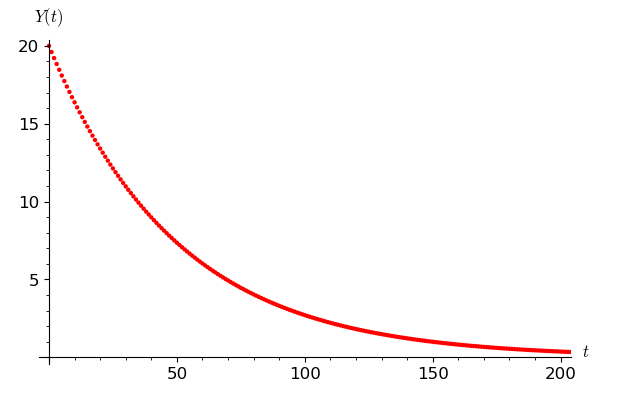
\includegraphics[scale = 0.7]{simulacao_Y.PNG} 
    \caption{Simulação da população de predadores}
    \label{fig:simulacao_Y}
\end{figure}

Na Figura \ref{fig:simulacao_I}, temos a simulação referente à população de presas infectadas.
\begin{figure}[H]
    \centering
    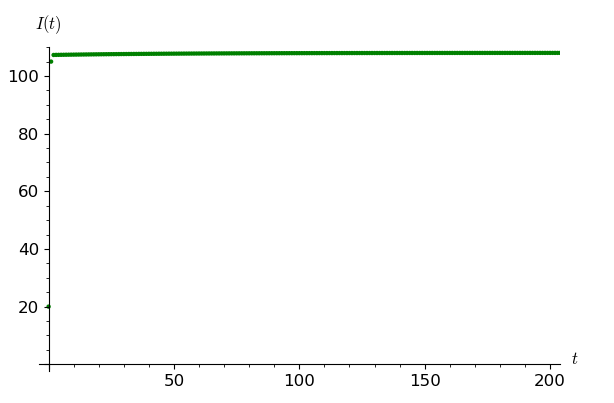
\includegraphics[scale = 0.7]{simulacao_I.PNG} 
    \caption{Simulação da população de presas infectadas}
    \label{fig:simulacao_I}
\end{figure}
\section{Discussão}
O parâmetro $r$ do modelo representa a taxa de crescimento da população de presas suscetíveis. Quanto maior $r$, mais rápido a população atinge o suporte do ecossistema. Para $r = + \infty$, podemos considerar $s + i = k$. Desse modo, o sistema reduz para duas dimensões, como apresentado na Equação \ref{eq:sist_bi}. Uma das conclusões obtidas no trabalho de modelagem por Joydev Chattopadhyay e Ovide Arino \cite{chattopadhyay} é que o comportamento assintótico do sistema tridimensional é muito próximo do modelo bidimensional obtido ao considerar $r = + \infty$.

A análise de estabilidade local pode ser realizada calculando-se as matrizes variacionais correspondentes a cada equilíbrio. Seja $V_0$ a matriz variacional referente a $E_0$. Temos que  
\begin{equation*}
    V_0 = 
    \begin{bmatrix}
        bk - c & 0 \\
        0 & -d \\
    \end{bmatrix},
\end{equation*}
e, consequentemente, os autovalores são $-d$ e $bk - c$. Seja $V_1$ a matriz variacional referente a $E_1$. Temos 
\begin{equation*}
    V_1 = 
    \begin{bmatrix}
        c - bk & - \upgamma(I^*) \\ 
        0 & \varepsilon \upgamma(I^*) - d \\
    \end{bmatrix},
\end{equation*}
sendo os autovalores da matriz $c-bk$ e $\varepsilon \upgamma(I^*) - d$. Seja $V_*$ a matriz variacional referente a $E_*$, assim,
\begin{equation*}
    V_* =
    \begin{bmatrix}
        - b I^* + \dfrac{\upgamma(I^*)Y^*}{I^*} - \upgamma'(I^*) Y^* & -\upgamma(I^*) \\
        \varepsilon \upgamma'(I^*)Y^* & 0 \\.
    \end{bmatrix}
\end{equation*}

A equação característica de $V_*$ é 
\begin{equation*}
    \lambda^2 - \lambda \left( \dfrac{\upgamma(I^*)Y^*}{I^*} - b I^* -  \upgamma'(I^*) Y^* \right) + \varepsilon \upgamma'(I^*)Y^*\upgamma'(I^*) = 0.
\end{equation*}

Sendo assim, é evidente que se $\left( \dfrac{\upgamma(I^*)Y^*}{I^*} - b I^* -  \upgamma'(I^*) Y^* \right) > 0$, o equilíbrio é instável. Se for menor que zero, o equilíbrio é estável. Ademais, é necessário que $k > \dfrac{c}{b}$ para que exista a componente $I^*$ do equilíbrio. Note que essa condição implica a existência do equilíbrio $E_1$. Desse modo, concluímos que a existência de $E_*$ implica a existência de $E_1$, porém o contrário não é válido.

Se o equilíbrio $E_1$ é localmente assintoticamente estável, a população de predador não vai persistir. Em contrapartida, a população infectada vai sobreviver. Na simulação realizada, utilizaram-se parâmetros de modo que $E_1$ fosse localmente assintoticamente estável. Nas figuras \ref{fig:simulacao_Y} e \ref{fig:simulacao_I}, é possível notar que a população de predadores é extinta, enquanto a população de presas cresce até atingir o suporte do ecossistema.

\section{Conclusão}
Analisamos um modelo tridimensional de uma dinâmica predador-presa afetando a população de presas. O modelo possui três espécies: presas suscetíveis, presas infectadas e predadores. Assumindo que a taxa de crescimento da população de presas, $r$, era $+ \infty$, transformamos um modelo tridimensional em bidimensional, sem perda significativa de resultados para o comportamento assintótico do primeiro. Posteriormente, encontramos os equilíbrios do sistema bidimensional e suas respectivas estabilidades.

Conforme comentado na Introdução, a abordagem aqui presente se mostra de grande importância, por conter modelagens significativamente próximas da realidade, apesar das limitações. Além disso, a abordagem mescla duas importantes áreas da Modelagem de Fenômenos Biológicos, possibilitando a expansão de ambas. Destaca-se, ainda, a escassez de artigos semelhantes, indicando o forte potencial de desenvolvimento do tema em questão.

Em trabalhos futuros, podem ser explorados os seguintes casos: a população de predadores também é afetada pela doença, uma parte da população de presas infectadas se recupera e retorna para a população de presas suscetíveis, e a doença é transmitida hereditariamente. 
\printbibliography
\end{document}
